\chapter{Image Signal Processing Pipeline}%

Producing a perceptually pleasing image involves several processing steps typically executed within the camera. These steps are orchestrated by a computing unit known as the Image Signal Processor (ISP). The tasks within the ISP are divided into distinct blocks, which can operate in parallel or series, depending on the specific processing requirements. Figure \ref{fig:dip} illustrates a typical colour image processing pipeline.

Each block in the pipeline has adjustable parameters that can be fine-tuned to meet specific preferences or requirements. Image quality experts are utilized in the industry to optimize these parameters and to perform experiments on subjective image quality, using, for example, ordinary people and their preferences.

\begin{figure}
\centering
\documentclass[tikz,border=10pt]{standalone}
\usepackage{xcolor}
\usepackage{tikz}

\begin{document}

\begin{tikzpicture}
    % Constants
    \def\boxWidth{1}
    \def\boxHeight{0.5}
    \def\numBoxes{11}
    \def\gammaValue{2.2} % Adjust this value for different gamma corrections

    % Draw the perceived brightness boxes
    \foreach \x in {0,...,\numBoxes}
    {   
        \pgfmathsetmacro\shade{(\x/\numBoxes)^(1/\gammaValue)}
        \definecolor{currentcolor}{rgb}{\shade,\shade,\shade}
        \fill[currentcolor] (\x*\boxWidth,0) rectangle ++(\boxWidth,\boxHeight);
        \draw (\x*\boxWidth,0) rectangle ++(\boxWidth,\boxHeight);
        \node at (\x*\boxWidth + 0.5*\boxWidth, 0.25*\boxHeight) {\tiny\pgfmathprintnumber[precision=1,fixed]{\x/\numBoxes}};
    }
    \node[anchor=east] at (0,0.25*\boxHeight) {Perceived (linear) brightness};

    % Draw the physical brightness boxes
    \foreach \x in {0,...,\numBoxes}
    {
        \pgfmathsetmacro\shade{\x/\numBoxes}
        \definecolor{currentcolor}{rgb}{\shade,\shade,\shade}
        \fill[currentcolor] (\x*\boxWidth,-1.5*\boxHeight) rectangle ++(\boxWidth,\boxHeight);
        \draw (\x*\boxWidth,-1.5*\boxHeight) rectangle ++(\boxWidth,\boxHeight);
        \node at (\x*\boxWidth + 0.5*\boxWidth, -1.25*\boxHeight) {\tiny\pgfmathprintnumber[precision=1,fixed]{\x/\numBoxes}};
    }
    \node[anchor=east] at (0,-1.25*\boxHeight) {Physical (linear) brightness};

\end{tikzpicture}

\end{document}

\caption{Simplified colour image processing pipeline. Adapted from \cite{Ramanath}, \cite{JianpingZhou2007IPTf}}
\label{fig:dip}
\end{figure}


\section{Black Level Subtraction}

Dark current is a noise source in photography, mostly prevalent at long exposures. This can be observed by covering the camera lens entirely with a lens cap so that no light is incident on the sensor so that one would expect it not to record any voltage. However, this is wrong as the temperature around the sensor may cause electrons to be emitted, so a signal is recorded within the sensor. This type of noise can be characterized by measuring the average signal recorded under an environment where no light is incident on the sensor. \cite[289]{nakamura}, \cite[63, chapter. 3]{rowlands2020physics} This type of noise can be characterized by taking images while the shutter is closed or by placing a lens cap in front of the camera so that no light enters inside, and thus, the noise source can be isolated \cite{Ramanath}. This is why it is often called \textbf{Black Level Subtraction} (BLS).

\section{Lens Shading Correction}

As was discussed in \ref{ss:optics}, lens shading results in the edges of the image having decreased brightness or variation in colour. The correction is typically performed by first characterizing the shading with a flat-field image, as was described before. As this flat-field image has to be saved on the device for correction purposes, it is often downsampled prior to characterization into a smaller size, e.g. $17 \times 13$, and interpolated at runtime. This process is thus called Lens Shading Correction (LSC).

Luminance shading can be fixed by generating an inverse of the captured flat-field image, where the entries are the gain factors that must be applied to achieve similar brightness as in the centre of the image. \cite[286-287]{nakamura}. Depending on the optical system, the corners may sometimes be drastically darker in the flat-field image, and correcting them entirely in the digital domain would result in noisy corners. As such, the lens shading correction might not remove the shading altogether.

On the other hand, colour shading requires generating a similar correction table, but for each channel separately. Since for a uniformly illuminated image, it would be expected that the colour channels would be equal at every pixel location, the correction table is typically derived as a relative measure to some other channel's value. \cite[286-287]{nakamura}. Since the green channel is typically the brightest in an image, often the table is generated by the ratio of red and blue values to the green values, $R/G$ and $B/G$.

\section{White Balance}

The concept of white balancing in cameras, as explained in \cite[ch.~4.6]{rowlands2020physics}, is employed to replicate the phenomenon of chromatic adaptation discussed in section \ref{sec:chromaticadaptation}. White balancing is achieved by estimating the illuminant present in the scene and employing pre-defined multipliers to the pixel values that would equal the red, green and blue responses for an object that appears white to a human. As each illuminant might result in different proportions of red, green and blue responses for an object that appears white to a human, these multipliers are computed for a set of distinct illuminant types. This process, combined with colour correction, cancels the effect of the illuminant and thus simulates the chromatic adaptation behaviour. 

The illuminant estimation algorithm primarily determines the accuracy of white balance algorithms. A wrong estimation results in an improper choice of multipliers for colour correction and white balance and a distinct tint in the output image. Thus, the illuminant estimation process is perhaps the most important in the colour processing pipeline. For a review on illuminant estimation algorithms, we refer the reader to \cite{colourconstancy}.

\section{Demosaic}

As discussed in Section \ref{ss:colour}, producing colour images begins with the image sensor being overlaid with a colour filter array. This array allows only light of specific wavelengths to pass through, a concept illustrated in \ref{fig:cfa}. The next step in creating a full-colour image involves a crucial process known as demosaicing.

Demosaicing employs various interpolation techniques to achieve colour accuracy. Among the simplest is bilinear interpolation, based on direct interpolation methods. However, as documented in practical applications, these simple algorithms can sometimes fail, particularly at image edges \cite[46]{Ramanath}.

Acknowledging these limitations, researchers have developed more sophisticated algorithms. These advanced methods leverage cross-correlations between channels, adaptive filters, and frequency information. Such enhancements significantly improve the performance of demosaicing algorithms. Interested readers may refer to \cite{gunturk2005demosaicking} for a more detailed discussion on this topic.


\begin{figure}
    \centering
    \pdftooltip{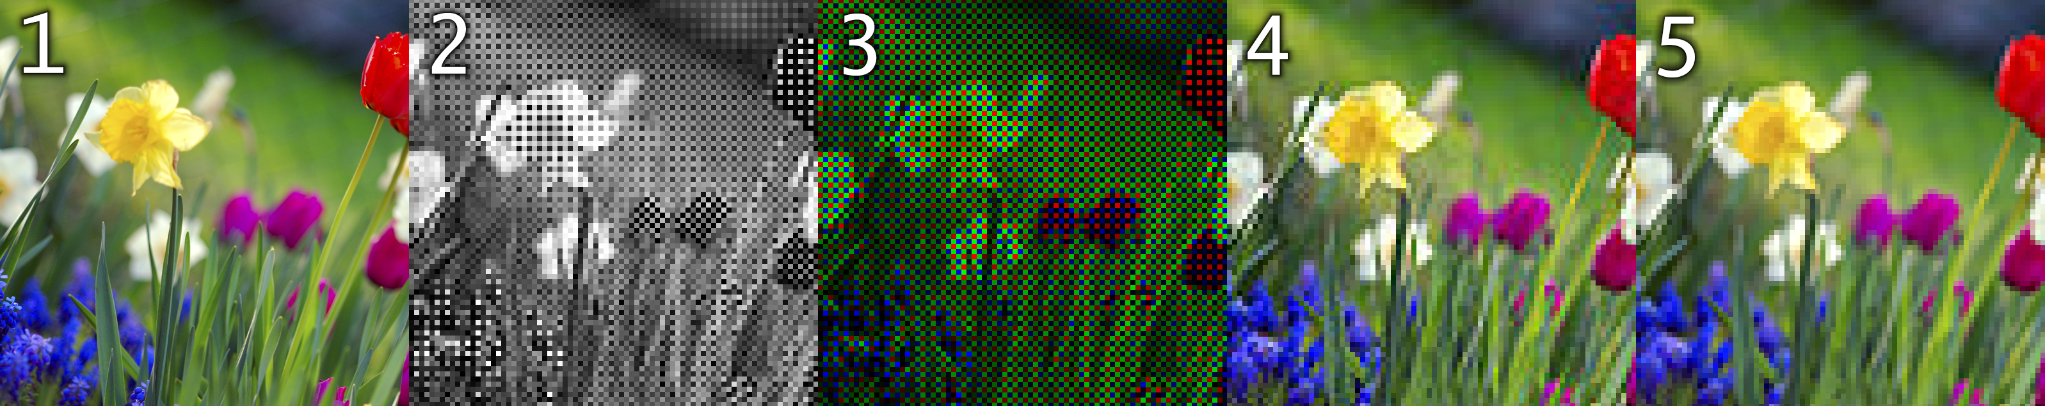
\includegraphics[width=\textwidth]{figures/horizontal_flowers.png}}{Demosaic process. Image copied from \cite{demosaic} under CC-BY-ND License.}
    \caption{Demosaic process \cite{demosaic}}
    \label{fig:demosaic}
\end{figure}

\section{Colour Correction}
 \label{ss:cc}
Figures \ref{fig:xyz} and \ref{fig:d5100} demonstrate the significant differences in spectral responsivities between the human eye and digital cameras, resulting in varying colour responses. Furthermore, the responsivities can vary across different units of the same camera module \cite{walowit2019best}. In addition to colour inaccuracy, it also results in observer metamerism, where the camera captures two objects that appear the same colour to the human eye differently.

A colour correction matrix is typically applied to the input image to account for the differences. The simplest way is to derive a 3x3 matrix by regression from camera responses to known XYZ responses for a standard observer. Like white balancing, this matrix is unique to each illuminant as white balancing only guarantees that neutral colours are mapped correctly \cite[1]{cheng2015beyond}. Furthermore, we can directly transform the input values to the desired output space with colour correction matrices, such as sRGB. This step is also often known as colour space transformation (CST).

\section{Gamma}


Finally, the image has to be saved for storage. At this stage, the image is likely still in linear colour space, such as linear sRGB, and has to be transformed through a non-linear inverse gamma function to compensate for the monitor gamma \cite{4050037}. The gamma function is often modelled as follows:

\begin{equation}
V_{\text{out}} = V_{\text{in}}^\gamma,
\end{equation}

where $V_{\text{out}}$ is the output voltage after applying the gamma function, $V_{\text{in}}$ is the input voltage and $\gamma$ is the so-called decoding gamma. The camera pipeline thus applies the reciprocal gamma $V_{\text{in}}^{\frac{1}{\gamma}}$ at encoding phase. 

Typically, the gamma is roughly $2.2$ to comply with colour spaces such as \cite{sRGB}. Inverse gamma was initially applied in images to compensate for non-linearities in CRT monitors. Still, it has also been found to closely simulate the human perception of brightness, which more accurately senses differences in darker tones. The input range becomes linear again when gamma decoding is performed on the monitor. When the image is viewed, the human eye performs its correction again, resulting in a similar perceived depth as stored.

\section{Post-processing}

In this phase, the process varies among different manufacturers, focusing more on enhancing the image's visual appeal and ensuring it meets the intended output specifications. At this stage, the objective shifts from faithfully recreating the original scene to crafting an image representing an ideal version of what was observed.

Typical algorithms employed at this stage enhance the colours, for instance, by making them look more saturated and removing artefacts such as noise from the image. Sharpness is typically preferred, so an additional edge sharpening step is often performed.  \cite[40-41]{Ramanath} \cite{4050037}

Before display, the image is often compressed to save space. This might discard information from the image that is not perceptually important to the viewer. Hence, they are often called lossy algorithms and convert the image into colour space with less correlation and detail across channels. Typical encoding formats encountered these days are some variants of JPEG \cite{JPEG} and PNG \cite{PNG}.